\subsection*{Supplemental Figures}
\setcounter{figure}{0} % set figs to start at 1
\renewcommand{\thefigure}{S\arabic{figure}} % start figures with "S"

% See 4maintextFigs.txt for functions and usage to help streamline making figures

%%%% tony %%%%
\begin{figure}[h]
\centering
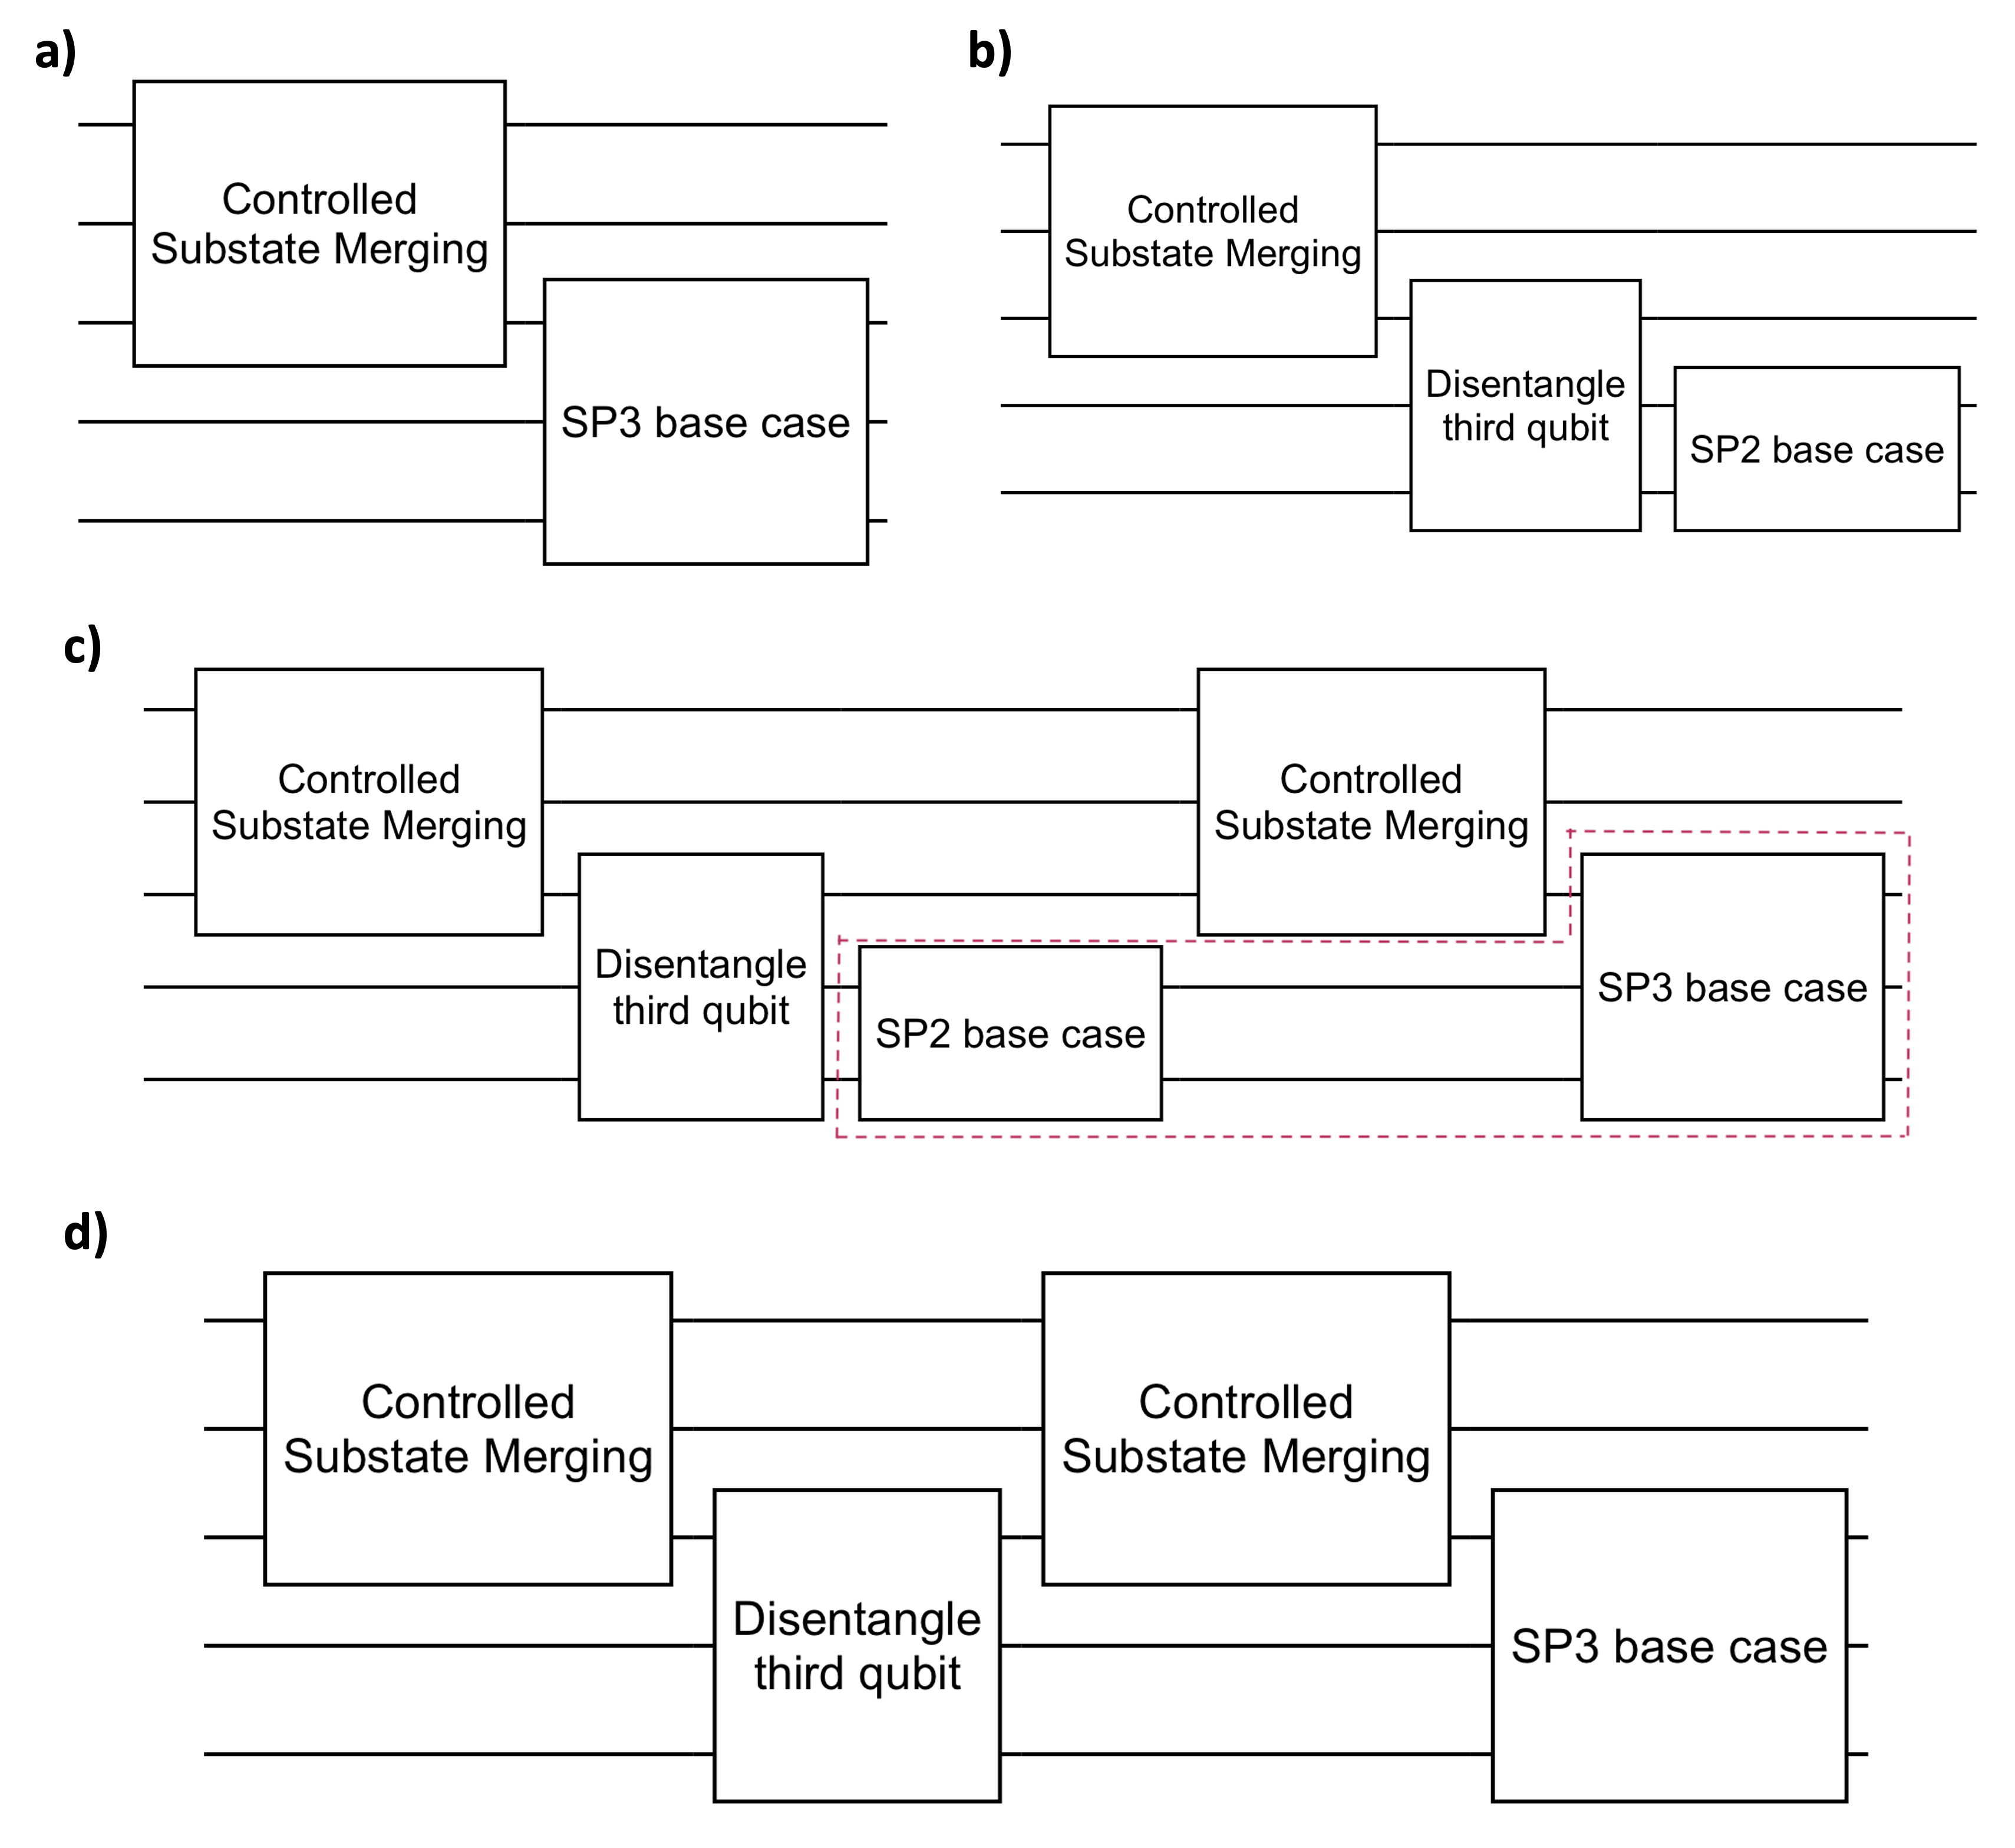
\includegraphics[width=0.95\linewidth]{main/figs/sfig_1.png}
\caption{Quantum circuit components comprising the ISA framework. a) General quantum circuit structure of a single iteration of ISA using a
two-bit pattern $p$. Several iterations of controlled substate merging are
performed on neighboring qubits before a three-qubit state preparation base case
is applied. b) Decomposition of a single iteration of ISA using a two-bit pattern $p$.
The three-qubit state preparation base case is broken down into a distangling
step and a two-qubit state preparation base case. c) General quantum circuit structure for two consecutive iterations of ISA
ending in a three-qubit base case on the same three qubits. Note that the SP2 
base case in the first ISA iteration can be commuted with the controlled substate
merging step in the second ISA iteration. d) General quantum circuit structure for two consecutive iterations of ISA
width the same three-qubit state preparation base case after applying retroactive
base case reduction. The SP2 block from Figure 4 is merged with the later SP3
block, saving 1 CX gate.}
\label{sfig1}
\end{figure}

\begin{figure}[h]
\centering
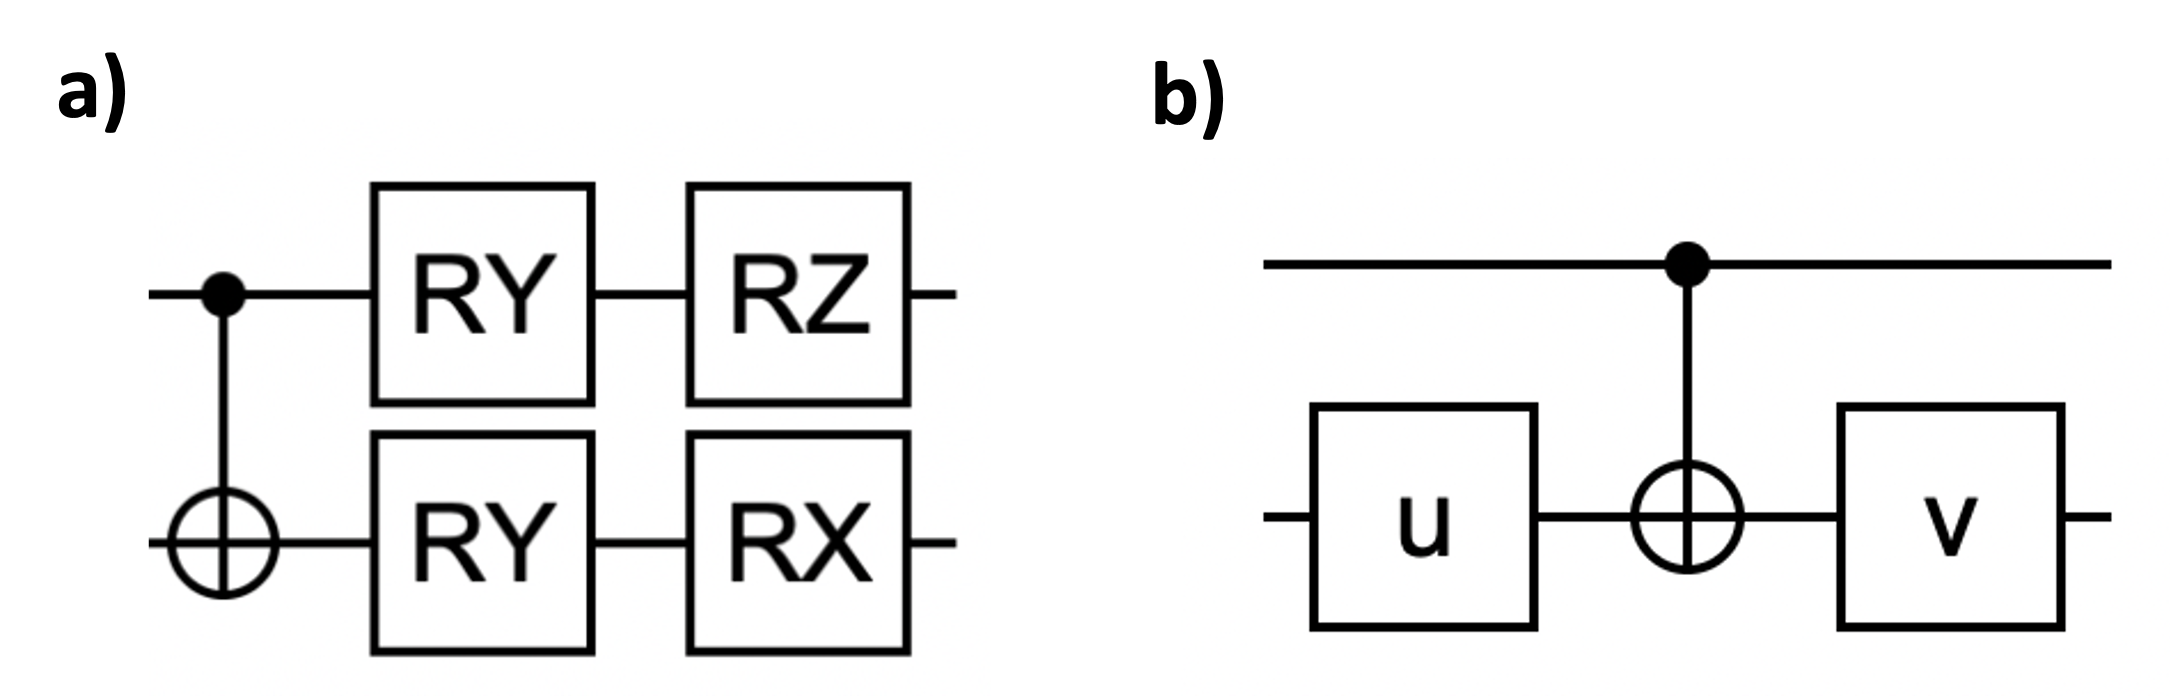
\includegraphics[width=0.6\linewidth]{main/figs/sfig_2.png}
\caption{a) The circuit block used in ADAPT-VQE for state preparation. The operator
pool was generated by translating this block across different pairs of 
adjacent qubits. Each operator contains four parameters, one for each rotation.
All four rotation angles were initialized to zero. b) Target decomposition of the uniformly controlled single-qubit rotation with one control qubit}
\label{sfig2}
\end{figure}



% \generateFig{tony}{tony}{.3} 
%     {This is a picture of Tony Capra}
%     {Nobody puts Tony in a supplement\dots}
% \tony

% %%%% cutegoat %%%%
% % Example of sideways figure

% \generateFig[90]{cutegoat}{cutegoat}{.6} % Make angle 90deg
%     {This cute sideways goat wishes you good luck with your manuscript} % bold caption
%     {This is how you rotate a figure but not the caption. To rotate the caption with the figure, use the function(s) \texttt{generateSidewaysFig} or \texttt{generateSidewaysFigSubpanels}.} % unbold caption
% \cutegoat

\clearpage